%  Typ dokumentu - článek, prezentace aj.
\documentclass[english]{article}

%  Nastaví vstupní a výstupní kódování znaků (encoding) a lokalizace
\usepackage[T1]{fontenc}
\usepackage[utf8]{inputenc}
\usepackage[english,czech]{babel}
\usepackage{icomma}

%  Formát papíru a odsazení od jeho okrajů
\usepackage[letterpaper]{geometry}
\geometry{verbose,tmargin=1.5cm,bmargin=2cm,lmargin=2cm,rmargin=2cm}

%  Umožňuje pracovat s grafikou
\usepackage{graphicx}
\usepackage{bigstrut}
\usepackage{epstopdf}

%  Automaticky odsadí i první paragraf v každé sekci
\usepackage{indentfirst}

%  Umožňuje rozdělovat obsah na více sloupců
\usepackage{multicol}
\usepackage{booktabs}
\usepackage{pgffor}

% physics
\newcommand{\unit}[1]{\ \mathrm{#1}}
\newcommand{\dd}{\mathrm{d}}
\newcommand{\ee}{\mathrm{e}}

%  Umožňuje používat hypertextové odkazy, nastavuje jejich barvu a
%  vlastnosti
\usepackage[unicode]{hyperref}
\hypersetup{
colorlinks=true, citecolor=blue, filecolor=blue, linkcolor=blue,
urlcolor=blue
}

%  Formátování stránek, empty = odstraní číslování
% \pagestyle{empty}

%  Řádkování
\linespread{1.2}

%  Lepší zobrazování matematiky (rozšíření sum o \limits atd.)
\everymath{\displaystyle}
\usepackage{amsmath, amsthm, amssymb}

% Umožní psát přes \mathbb{N/R/Q/..} množiny čísel
\usepackage{amssymb}

%  Velikost fontu matematických výrazů v dokumentu lze pro danou
% základního fontu dokumentu upravit pomocí:
% \DeclareMathSizes{X}{Y}{Z}{U} kde:
% X je velikost fontu v dokumentu, pro kterou se matematika upraví
% Y je standartní velikost fontu matematiky
% Z je velikost fontu zmenšených (vnořených výrazů)
% U je velikost fontu ještě více zmenšených (vnořených výrazů).
\DeclareMathSizes{10}{10.5}{9}{9}

%  Nastaví autora, název, datum, skupinu měření apod. (můj vlastní
% příkaz, umožní znovu-použití v dokumentu)
\newcommand{\Author}{David Roesel}
\newcommand{\Coauthor}{Hystereza Schönfeldová}
\newcommand{\Institute}{FJFI ČVUT v Praze}
\newcommand{\Subject}{FYZIKÁLNÍ PRAKTIKUM II}
\newcommand{\Group}{7}
\newcommand{\Circle}{ZS 7}
\newcommand{\Title}{Úloha \#2  \\Měření hysterezní smyčky balistickým galvanometrem}
\newcommand{\Date}{14.4.2014}

% Začátek dokumentu - Formátování na výstup
\begin{document}

% Interní proměnné, možno zobrazovat u prezentací, používají se při
% generování pomocí \titlepage apod.
\author{\Author}
\title{\Title}
\date{\Date}

%  Lokalizace některých názvů do češtiny
\renewcommand{\figurename}{Obr.}
\renewcommand{\tablename}{Tab.}
\renewcommand{\refname}{Reference}

% --- Hlavička dokumentu -----------------------------------------------

\setlength{\parindent}{0cm}
\begin{multicols}{2}
\textbf{\Subject \\
        \Institute \\[0.1cm]
%\large  \Title \\[0.5cm]
\Title \\[0.5cm]
}
\begin{tabular}{rlrl}
\large Datum měření: & \Date & \large Skupina: & \Group \\
\large Jméno: & \Author & \large Kroužek:  & \Circle\\
\large Spolupracovala: & \Coauthor &\large Klasifikace:\\
\end{tabular}

\begin{flushright}

\includegraphics[scale=0.28]{../../_meta/fjfi_standart.pdf}
\hspace{0.2cm}

\includegraphics[scale=0.28]{../../_meta/cvut_standart.pdf}
\end{flushright}
\end{multicols}
\hrule
\vspace{0.5cm}

% ----------------------------------------------------------------------


% --- Tělo dokumentu ---------------------------------------------------
\setlength{\parindent}{0.5cm}
\section{Pracovní úkoly}
\begin{enumerate}
\item Změřte hysterezní smyčku toroidu z dané feromagnetické látky a graficky ji znázorněte.

\item Určtete koercitivní sílu $H_K$ a remanenci $B_R$.

\item Diskutujte, jak magnetické pole země ovlivňuje měření a zda-li je možné jej s danou aparaturou měřit.
\end{enumerate}

	
\section{Vypracování}

	\subsection{Použité přístroje}
		Balistický galvanometr, odporová dekáda, aparatura s toroidem, vypínačem a nastavitelným odporem, 2 přepínače, komutátor, digitální multimetr, stabilizovnaý zdroj, normál vzájemné indukčnosti, vodiče.
	
	\subsection{Teoretický úvod}
		Pomocí hysterezní křivky vyjadřujeme závislost magnetické indukce $B$ ve studovaném feromagnetiku na intenzitě vnějšího magnetického pole $H$. Během úlohy budeme používat pro měření této křivky balistického galvanometru (schéma převzaté z \cite{bib:zadani} je na Obr.~\ref{fig:schema}). 
		
		Měřit budeme toroid z feromagnetického materiálu, na kterém je navinuta cívka. Bude-li touto cívkou procházet proud, bude tím vytvářet magnetické pole $H$. Magnetickou indukci $B$ ve zkoumaném vzorku můžeme zkoumat pomocí měrné cívky v obvodu za pomoci balistického galvanometru.  
		
		Za jistých předpokladů můžeme jinak složitě popsatelný průběh magnetického pole uvnitř vzorku aproximovat. Používáme-li hustě vinutý toroid, budou magnetické siločáry nabývat tvaru kružnic, které budou ležet v rovinách kolmých k rotační ose toroidu a jejich středy budou ležet v této ose. Intenzita magnetického pole bude mít stejnou velikost podél celé siločáry. Jako další z předpokladů bereme, že šířka toroidu bude mnohem menší, než poloměr jeho střední kružnice, což nám dovoluje uvažovat v toroidu magnetické pole homogenní. Platit pro něj potom bude
		
		\begin{equation} \label{eq:Hfinal}
		H = \frac{n_1 I}{2 \pi r},
		\end{equation}
		kde $n_1$ je počet závitů magnetizační cívky, $I$ je proud v ní procházející a $r$ je poloměr střední kružnice toroidu.
		
		
		Pro magnetickou indukci v toroidu platí
		\begin{equation}
		B = \frac{\Phi}{N_2 S},
		\end{equation}
		kde $\Phi$ je magnetický tok procházející cívkou, $N_2$ je počet závitů cívky a $S$ její průřez. Vzhledem k tomu, že měříme magnetizační tok toroidu, nevznikají žádné póly a nemusíme uvažovat jejich demagnetizační vliv.
		
		Změna magnetické indukce se tím pádem rovná
		\begin{equation}
		\Delta B = B_1 - B_2 = \frac{\Phi_1 - \Phi_2}{N_2 S}.
		\end{equation}
		% %
		Faradayův zákon nám dává vztah
		\begin{equation}
		-\frac{\dd \Phi}{\dd t} = U = R\cdot I,
		\end{equation}
		kde $U$ a $I$ jsou napětí a proud v měřené cívce a $R$ je odpor obvodu s galvanometrem.
		
		Jde o rovnici, která se dá řešit separací. Pro časový interval $t_1$ -- $t_2$ za změny magnetického indukčního toku v intervalu $\Phi_1$ -- $\Phi_2$ dostáváme
		\begin{equation}
		\int_{\Phi_1}^{\Phi_2} \dd \Phi = -R \int_{t_1}^{t_2} i \dd t.
		\end{equation}
		
		
		V případě, že je $Q = \int_{t_1}^{t_2}i\dd t$ celkový náboj, který projde balistickým galvanometrem, bude platit
		\begin{equation}
		\Phi_1 - \Phi_2 = R Q.
		\end{equation}
		Pro tento náboj dále platí
		\begin{equation}
		Q = K_b \lambda s_1,
		\end{equation}
		kde $K_b$ je balistická konstanta, $\lambda$ činitel závislý na tlumení galvanometru a $s_1$ balistická výchylka redukovaná na délku kruhového oblouku.
		
		Pro změnu magnetické indukce $\Delta B$ tedy celkově dostáváme
		\begin{equation} \label{eq:deltaBfial}
		\Delta B = \frac{R K_b\lambda s_1}{N_2 S}.
		\end{equation}
		% %
		
		Pro výpočet ale potřebujeme zjistit členy $K_b$ a $\lambda$, což provedeme cejchováním galvanometru. Budeme-li komutovat proud $I_1$, který prochází primární cívkou normálu vzájemné indukčnosti, bude před komutací magnetický indukční tok sekundární cívkou roven $\Phi_1 = L_{12}I_1$ a po komutaci $\Phi_2 = - L_{12}I_1$. Celkovou změnu indukčního toku, která v galvanometru kumuluje náboj $Q_1$, můžeme zapsat ve tvaru $\Delta \Phi = 2 L_{12} I_1$. Pro tento náboj tím pádem dostáváme dva vztahy
		\begin{equation}
		2 L_{12} I_1 = R Q_1, \qquad Q_1 = K_b \lambda s_1^*
		\end{equation}
		a celkem
		\begin{equation} \label{eq:rkblambda}
		R K_b \lambda = \frac{2 L_{12} I_1}{s_1*}.
		\end{equation}
		
		\begin{figure}[hbt]
		\centering
		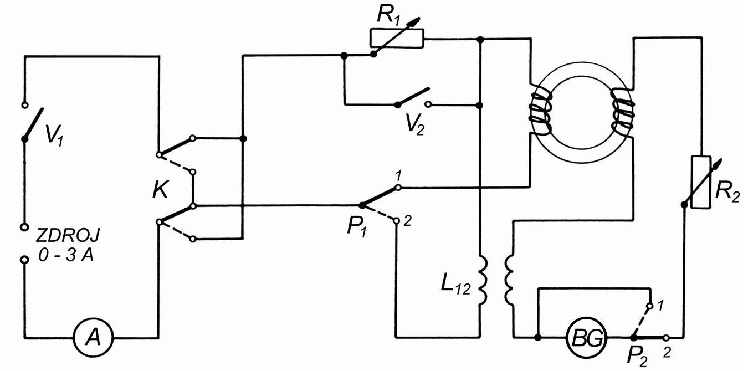
\includegraphics[width=0.5\textwidth]{att/schema.pdf}
		\caption{Schéma zapojení. Převzato z \cite{bib:zadani}. }
		\label{fig:schema}
		\end{figure}
				
	\subsection{Postup měření}
		% %
		Vzhledem k nefunkční aparatuře jsme dostali referenční naměřené hodnoty. Úlohu jsme se však snažili usilovně měřit celé praktikum a postupovali jsme podle následujícího postupu. 
		
		Aparaturu jsme zapojili podle zadání, tedy dle Obr. \ref{fig:schema}. Zdroj napětí jsme nastavili tak, abychom dosahovali maximálně 600~mA. V našem nastavení aparatury se nepovedlo dostat na nižší hodnotu než 15~mA. Jako odpor $R_2$ jsme dle zadání zapojili dekádu a nastavili na ní takový odpor, aby při proudu $I_{max}$, zapnutém vypínači $V_2$ a přepínači $P_1$ v poloze 1 byla značka balistického galvanometru stále na stupnici. V našem případě se jednalo o $R_2 = 20$~k$\Omega$, což ale nemusí odpovídat námi zpracovávaným datům. Proud $I_{max}$ jsme podle zadání volili 600~mA a během měření jsme se ujišťovali, že se hodnota nezměnila, abychom proměřovali stále stejnou hysterezní smyčku.
		
		\begin{figure}[hbt]
		\centering
		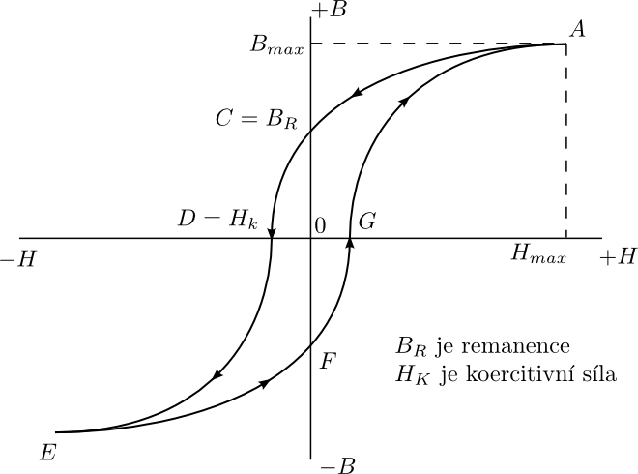
\includegraphics[width=0.5\textwidth]{att/hysterezni_smycka.pdf}
		\caption{Teoretická podoba hysterezní smyčky. Převzato z \cite{bib:zadani}}
		\label{fig:hysterezni_smycka}
		\end{figure}
		
		Nejprve jsme provedli cejchování balistického galvanometru. Přepínač $P_1$ jsme nechali v poloze 2 a na zdroji jsme nastavili nějaký proud v rozsahu 0 -- 600~mA. Poté jsme několikrát komutovali proud a zaznamenávali jsme výchylky na galvanometru $s_1^*$ a $s_1^{**}$ v obou směrech. Aritmetickým průměrem pak spočítáme závěrečnou hodnotu výchylky (výchylky $s_1^*$ i $s_1^{**}$ by měly být při každém měření téměř stejné).
		
		Měření jsme dále prováděli podle následujících kroků (za používání značení z Obr. \ref{fig:hysterezni_smycka}). 
		
		\begin{itemize}
			\item \emph{Proměřování úseku A--C}: Přepínač $P_1$ dáme do polohy 1. Vypínač  $V_2$ vypneme a skrze změny odporu $R_1$ nastavíme určitou hodnotu proudu od 0 do $I_{max}$. Poté vypínač $V_2$ zapneme a několikrát komutujeme proud pomocí komutátoru $K$, čímž pokaždé proběhneme hysterezní smyčku. Jednu z poloh komutátoru ''nahoře`` určíme jako odpovídající bodu $A$ (opačná tím pádem bude odpovídat bodu $E$) a tu nastavíme. Vypnutím vypínače $V_2$ rychle změníme hodnotu proudu z $I_{max}$ na předem stanovené $I$. To nám dá možnost změřit výchylku na galvanometru $s_1$, kterou odečteme a zaznamenáme. Před každým vypnutím $V_2$ počkáme, než se ukazatel galvanometru ustálí na nulové pozici. Celý postup opakujeme pro více hodnot stanoveného proudu $I$ (tedy bodů křivky). 
		
			\item \emph{V bodě C}: Místo $V_2$ vypneme přímo vypínač $V_1$ a vůbec nenastavujeme odpor $R_1$. 
		
			\item \emph{Proměřování úseku C--E}: Postupujeme analogicky, jen při vypínání $V_2$ zároveň komutujeme.
		
			\item \emph{Proměřování úseku E--F}: Postup identický s tím pro úsek \emph{A--C}, jen se změní počáteční poloha komutátoru na polohu ''dole``.
		
			\item \emph{V bodě F}: Postup identický jako u \emph{C}, jen se změní počáteční poloha komutátoru na polohu ''dole``.
		
			\item \emph{Proměřování úseku F--A}: Opět postupujeme stejně jako na úseku C--E, jen bude komutátor nastaven na polohu ''dole`` a během vypínání $V_2$ budeme komutovat na polohu ''nahoře``.
		\end{itemize}
		
		V průběhu celého měření neměníme odpor $R_2$, závisí na něm totiž absolutní výchylka galvanometru (tedy to, kterou hysterezní křivku proměřujeme).
		
		K zapojení galvanometru do obvodu využíváme přepínače $P_2$. Pokud zrovna chceme nastavovat proud, případně komutovat před vlastním měřením, můžeme díky němu regulovat tlumení galvanometru.		
				
		\subsection{Naměřené hodnoty}
			Vzhledem k tomu, že námi naměřené hodnoty nestačily ke kompletnímu vypracování úlohy, uvádíme pouze obdržená referenční data. Konstanty vystupující v našich výpočtech jsme brali v úvahu následovné: $r=17,1~\unit{mm}$, $N_1=62$, $N_2=400$, $L_{12}=7,27~\unit{mH}$ a $S=24,3~\unit{mm^2}$.
			
			Naměřené hodnoty z cejchování balistického galvanometru jsou uvedeny v Tab.~\ref{tab:data}. Z nich jsme pomocí vztahu~(\ref{eq:rkblambda}) dopočítali veličinu $RK_b^{(\rho)}\lambda$ a určili její velikost i s chybou spočítanou podle (\ref{eq:chyba_aritmetickeho_prumeru}) na 
			\begin{equation}
					RK_b^{(\rho)}\lambda = (0,3\pm0,1)~\unit{\frac{HA}{m}}.
			\end{equation}
			
			Zbytek naměřených hodnot, které uvádíme v Tab.~\ref{tab:data}, jsme zpracovali a vynesli do grafu na Obr.~\ref{fig:g_hyst}. Z nastavovaných proudů $I$ jsme pomocí vztahu~(\ref{eq:Hfinal}) spočítali hodnoty intenzity magnetického pole $H$. Pomocí vztahu~(\ref{eq:deltaBfial}) jsme ze spočítaného $RK_b^{(\rho)}\lambda$ dopočítali finální hodnoty změny magnetické indukce $\Delta B$, čímž jsme získali body námi studované závislosti. Přímo z naměřených hodnot jsme mohli odečíst remanenci, kterou jsme určili i s chybou podle (\ref{eq:chyba_neprime_mereni}) jako  
			\begin{equation}
					B_R = (1,0\pm0,4)~\unit{T},
			\end{equation}
			přičemž jsme uvažovali chybu změření výchylky $\sigma_s=0,1$ cm.
			K zjištění koercitivní síly jsme určili lineární extrapolací dvou nejbližších hodnot k ose x přibližný průsečík hysterezní křivky s touto osou. Finální hodnotu koercitivní síly tedy odhadujeme i s chybou na 
			\begin{equation}
					H_K = (15\pm5)~\unit{A/m}.
			\end{equation}
			

			
	\subsection{Diskuse}
			Vzhledem k tomu, že jsme zpracovávaná data neměřili my, nemůžeme dost dobře diskutovat jejich přesnost, případně možné chyby měření. Z námi provedených měření však bylo patrné, že jádrem celé úlohy je relativně nestabilní zdroj napětí, které značně kolísalo. Některé ze součástek  v obvodu už byly trochu starší a není jisté, jak moc se na ně dalo spolehnout. Z časových důvodů také při měření není možné čekat na dokonalé ustálení ukazatele balistického galvanometru a to do měření zanáší, ač malou, další chybu. Balistický galvanometr se také měl tendenci sám od sebe vychylovat z rovnovážné polohy a ta se v průběhu našeho měření změnila až o centimetr. 
			
			Jak v námi naměřených hodnotách, tak ve zpracovávaných datech byl znatelný rozdíl v hodnotách $RK_b^{(\rho)}\lambda$ určených při cejchování galvanometru. Finální hodnotu by šlo zpřesnit provedením více měření a tím pádem průměrováním většího počtu hodnot. Chyba při určování této konstanty však nezmění nic než sklon hysterezní smyčky, takže by na číselné výsledky neměla mít velký vliv. 
			
			Hodnota remanence se dá určit poměrně přesně, avšak velikost koercitivní síly je opravdu pouze odhadem z lineárního propojení nejbližších bodů. Stejně tak je obtížné dobře odhadnout velikost chyby této hodnoty. Jak remanence, tak koercitivní síla při tomto experimentu navíc záleží na posunutí hysterezní smyčky ve směru osy $y$, které jsme prováděli čistě z aritmetických průměrů extrémů naměřených hodnot a z předpokladu, že musí být hodnoty extrémů hysterezní smyčky symetrické podle os $x$ i $y$. Experiment nás však s hysterezní smyčkou dobře seznámil.
			
			Teoreticky by naše měření mohlo ovlivňovat magnetické pole Země. Jeho povrchová intenzita se však pohybuje mezi 24 až 66 $\unit{\mu T}$ \cite{bib:magpole}, což je zcela jistě pod rozlišovací schopnosti naší aparatury. Z tohoto důvodu není možné účinek magnetického pole Země změřit.
			
			
\section{Závěr}
		Změřili jsme hysterezní smyčku toroidu z dané feromagnetické látky a graficky jsme ji znázornili.
		
		Určili jsme koercitivní sílu $H_K$ a remanenci $B_R$ a buď vypočítali, nebo se pokusili odhadnout jejich chyby.
		
		Diskutovali jsme, jak magnetické pole země ovlivňuje měření a zda-li je možné jej s danou aparaturou změřit.		
	
\section {Použitá literatura}
% --- Literatura a reference -------------------------------------------
\begingroup
\renewcommand{\section}[2]{}

\begin{thebibliography}{9}
\bibitem{bib:zadani} Kolektiv KF, \emph{Návod k úloze: Měření hysterezní smyčky balistickým galvanometrem} [Online], [cit. \today] \newline http://praktikum.fjfi.cvut.cz/pluginfile.php/415/mod\_resource/content/3/HystSmycka\_2012v2.pdf

%\bibitem{bib:h3} Petr Chaloupka, \emph{Jak zpracovávat data} [Online], [cit. \today] \newline  https://dl.dropboxusercontent.com/u/11296940/zfm/h3.pdf

%\bibitem{bib:navody} Kolektiv KF, \emph{Návody k přístrojům} [Online], [cit. \today] \newline http://praktikum.fjfi.cvut.cz/documents/chybynav/navody-o.pdf

\bibitem{bib:chyby} Kolektiv KF, \emph{Chyby měření} [Online], [cit. \today] \newline http://praktikum.fjfi.cvut.cz/documents/chybynav/chyby-o.pdf

%\bibitem{bib:ctverce} Kolektiv KACH UPOL, \emph{Hodnocení analytických výsledků} [Online], [cit. \today] \newline http://ach.upol.cz/ucebnice/hodnoceni7.htm

\bibitem{bib:tabulky} J. Mikulčák a kol., Matematické, fyzikální a chemické tabulky \& vzorce. Prometheus,
Praha 2009.\newline
ISBN 978-80-7196-264-9

%\bibitem{bib:tlak} Český hydrometeorologický ústav, \emph{Měření tlaku} [Online], [cit. 7. dubna 2014] \newline http://portal.chmi.cz/files/portal/docs/poboc/OS/KW/Captor/tmp/DMULTI-P1PKAR01.gif

%\bibitem{bib:repo} Kolektiv autorů, \emph{Repozitář zdrojů k praktiku} [Online], [cit. \today] \newline  http://github.com/roesel/praktika

\bibitem{bib:magpole} geomag.bgs.ac.uk, \emph{The Earth's Magnetic Field: An Overview} [Online], [cit. \today] \newline http://www.geomag.bgs.ac.uk/education/earthmag.html

\end{thebibliography}
\endgroup
% ----------------------------------------------------------------------
\setcounter{equation}{0}
\numberwithin{equation}{section}
%\clearpage
\part*{Přílohy}

\section{Domácí příprava}
	Domácí příprava je přiložena k protokolu.
%\clearpage
\section{Statistické zpracování dat}

	Pro statistické zpracování využíváme aritmetického průměru:
	\begin{equation} \label{eq:aritmeticky_prumer}
	\overline{x} = \frac{1}{n}\sum\limits_{i=1}^{n}x_i,
	\end{equation}
%
%	jehož směrodatnou odchylku spočítáme jako 
%	\begin{equation} \label{eq:smodch_aritmetickeho_prumeru}
%	\sigma_0 = \sqrt{\frac{1}{n} \sum\limits_{i=1}^{n}\left( x_i - \overline{x} \right)^2 },
%	\end{equation}
%	
%	kde $ x_i $ jsou jednotlivé naměřené hodnoty, $ n $ je počet měření, $ \overline{x} $ aritmetický průměr a $ \sigma_0 $ jeho chyba \cite{bib:chyby}.
	
	
	jehož chybu spočítáme jako 
	\begin{equation} \label{eq:chyba_aritmetickeho_prumeru}
	\sigma_0 = \sqrt{\frac{1}{n(n-1)} \sum\limits_{i=1}^{n}\left( x_i - \overline{x} \right)^2 },
	\end{equation}
	
	kde $ x_i $ jsou jednotlivé naměřené hodnoty, $ n $ je počet měření, $ \overline{x} $ aritmetický průměr a $ \sigma_0 $ jeho chyba \cite{bib:chyby}.
	
Při nepřímém měření počítáme hodnotu s chybou dle následujících vztahů:
	\begin{equation}
	u = f(x, y, z, \ldots),
	\end{equation}
	\begin{displaymath}
	x = (\overline{x} \pm \sigma_x), \qquad
	y = (\overline{y} \pm \sigma_y), \qquad
	z = (\overline{z} \pm \sigma_z), \qquad
	\ldots,
	\end{displaymath}
	
	kde $ u $ je veličina, kterou určujeme nepřímo z měřených veličin $ x, y, z, \ldots $ 
	
	Pak
	\begin{displaymath}
	\overline{u} = f(\overline{x}, \overline{y}, \overline{z}, \ldots),
	\end{displaymath}
	\begin{equation}\label{eq:chyba_neprime_mereni}
	\sigma_u = \sqrt{\left( \frac{\partial f}{\partial x} \right)^2 \sigma^2_x + \left( \frac{\partial f}{\partial y} \right)^2 \sigma^2_y + \left( \frac{\partial f}{\partial z} \right)^2 \sigma^2_z + \ldots},
	\end{equation}
	\begin{displaymath}
	u = (\overline{u} \pm \sigma_ u).
	\end{displaymath}

%V případě, že máme několik různě přesných měření stejné veličiny, používáme vztah pro vážený průměr:
%	\begin{equation} 
%	\overline{x}=\frac{\sum\limits_{i=1}^{n}p_{i}x_{i}}{\sum\limits_{i=1}^{n}p_{i}},
%	\end{equation}
%	
%	kde $\overline{x}$ je vážený průměr, $x_{i}$ jsou jednotlivá měření a pro $p_{i}$ platí
%	 
%	\begin{equation}
%	p_{i}=\frac{1}{\sigma_{i}^{2}},
%	\end{equation}
%	
%	kde $\sigma_{i}$ jsou jednotlivé chyby daných měření.
%	 
%	Celkovou chybu tedy vypočítáme ze vztahu
%	\begin{equation} \label{eq:vazeny_prumer}
%	\sigma_{0}=\sqrt{\frac{1}{\sum\limits_{i=1}^{n}p_{i}}}.
%	\end{equation}
%
%\subsubsection{Metoda nejmenších čtverců}
%Snažíme-li se metodou nejmenších čtverců proložit data lineární závislostí $Y_i = ax_i+b$, dosazujeme hodnoty $x_i, y_i$ a snažíme se najít parametry $a$ a $b$ tak, aby byl součet všech kvadratických odchylek $\Delta Y_i^2$ minimální. Toho dosáhneme pomocí následujících vzorců \cite{bib:ctverce} :
%\begin{equation}\label{eq:ctverce_a}
%		a = \frac{n\sum\limits_{i=1}^{n}{x_i y_i}  - \sum\limits_{i=1}^{n}{x_i}\sum\limits_{i=1}^{n}{y_i}}{n\sum\limits_{i=1}^{n}{x_i^2}  - \left(\sum\limits_{i=1}^{n}{x_i}\right)^2}, \qquad \qquad
%		\sigma_a = \sqrt{\frac{n\sum\limits_{i=1}^{n}{(y_i - Y_i)^2} }{(n-2)\left(\sum\limits_{i=1}^{n}{x_i^2}  - \left(\sum\limits_{i=1}^{n}{x_i}\right)^2\right)}},
%\end{equation}
%
%\begin{equation}\label{eq:ctverce_b}
%		b = \frac{\sum\limits_{i=1}^{n}{x_i^2} \sum\limits_{i=1}^{n}{y_i}  - \sum\limits_{i=1}^{n}{x_i}\sum\limits_{i=1}^{n}{x_i y_i}}{n\sum\limits_{i=1}^{n}{x_i^2}  - \left(\sum\limits_{i=1}^{n}{x_i}\right)^2}, \qquad \qquad
%		\sigma_b = \sqrt{\frac{\sum\limits_{i=1}^{n}{x_i^2}\sum\limits_{i=1}^{n}{(y_i - Y_i)^2} }{n(n-2)\left(\sum\limits_{i=1}^{n}{x_i^2}  - \left(\sum\limits_{i=1}^{n}{x_i}\right)^2\right)}}.
%\end{equation}
%\section{Nákresy a schémata}
%			\begin{figure}[h!]
%			\centering
%			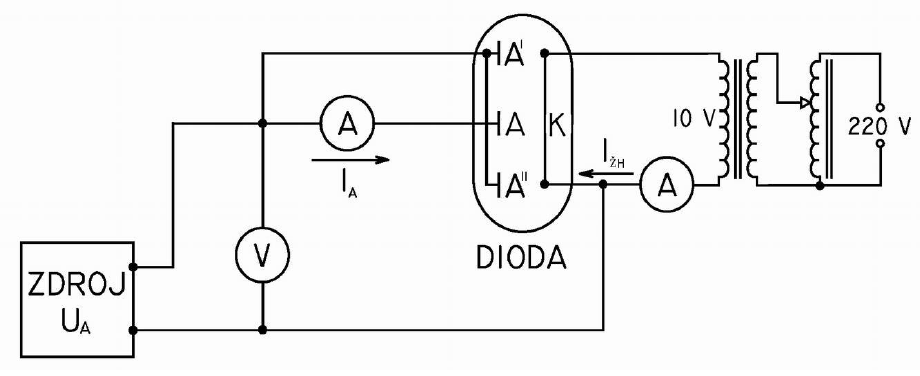
\includegraphics[width=12cm]{att/pyromet2.png}
%			\caption{Zapojení pro měření náběhového proudu. Převzato z \cite{bib:zadani}.}
%			\label{fig:s_aparatura_nasyc}
%			\end{figure}	
%			
%			\begin{figure}[h!]
%			\centering
%			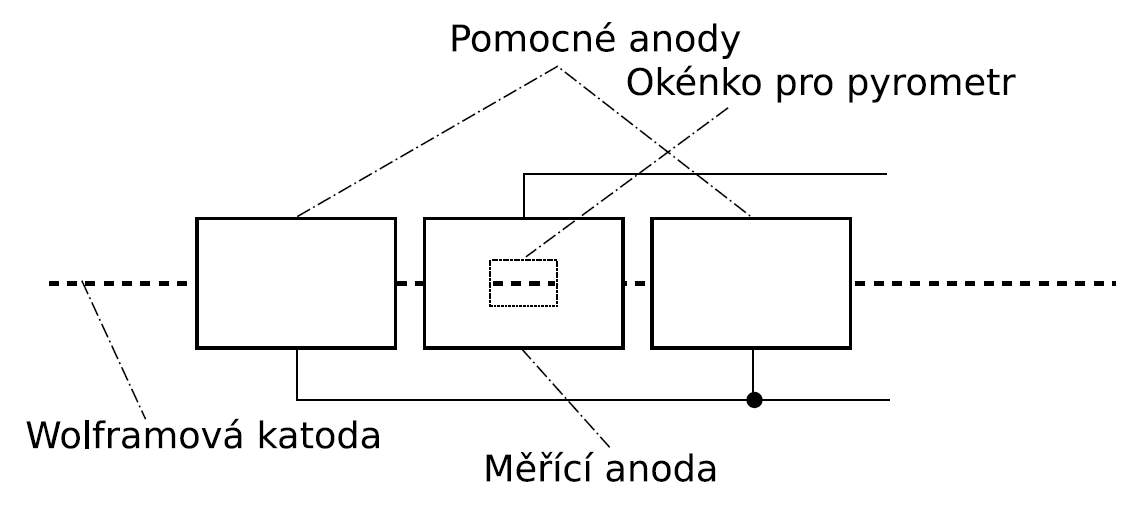
\includegraphics[width=10cm]{att/pyromet.png}
%			\caption{Geometrie uspořádání vakuové diody s pomocnými anodami pro dosažení homogenního pole. \newline Převzato z \cite{bib:zadani}.}
%			\label{fig:s_dida}
%			\end{figure}
%	
\clearpage
\section{Tabulky a grafy}

% Table generated by Excel2LaTeX from sheet 'List1'
\begin{table}[htbp]
  \centering
    \begin{tabular}{|r|r|r|r|r|r|}
    \hline
    \textbf{I [mA]} & \textbf{x [mm]} & \textbf{I [mA]} & \textbf{x [mm]} & \boldmath{}\textbf{$RK_b^{(\rho)}\lambda_1~\unit{[HA/m]}$}\unboldmath{} & \boldmath{}\textbf{$RK_b^{(\rho)}\lambda_2~\unit{[HA/m]}$}\unboldmath{} \bigstrut\\
    \hline
    331   & -9    & 351   & 8     & -0,53 & 0,64 \bigstrut\\
    \hline
    714   & -142  & 718   & 145   & -0,07 & 0,07 \bigstrut\\
    \hline
    576   & -82   & 576   & 83    & -0,10 & 0,10 \bigstrut\\
    \hline
    \end{tabular}%
  \caption{ Zpracovávané hodnoty cejchování balistického galvanometru; $I$ je stanovený proud, $x$ výchylka odečtená z galvanometru, $RK_b^{(\rho)}\lambda_{1,2}$ z jednotlivých měření dopočítávaný hledaný činitel.  }
  \label{tab:cejch}%
\end{table}%
 
			
% Table generated by Excel2LaTeX from sheet 'List1'
\begin{table}[htbp]
\catcode`\-=12 % HAX na enable cline v českym bable
  \centering
\begin{tabular}{|r|r|r|r|r|r|r|r|}
\hline
\multicolumn{2}{|c|}{$A\rightarrow D$} & \multicolumn{2}{c|}{$D\rightarrow A$} & \multicolumn{2}{c|}{$A\rightarrow D$} & \multicolumn{2}{c|}{$D\rightarrow A$} \bigstrut\\
\hline
\textbf{I [mA]} & \textbf{x [cm]} & \textbf{I [mA]} & \textbf{x [cm]} & \textbf{H [A/m]} & \textbf{B [T]} & \textbf{H [A/m]} & \textbf{B [T]} \bigstrut\\
\hline
612   & 0,0   & 610   & 19,2  & 353,16 & 2,52  & 352,00 & 2,49 \bigstrut\\
\hline
-612  & -18,9 & -24   & 4,6   & -353,16 & -2,41 & -13,85 & -1,32 \bigstrut\\
\hline
524   & -0,3  & -32   & 4,3   & 302,38 & 2,44  & -18,47 & -1,40 \bigstrut\\
\hline
403   & -0,7  & -54   & 3,6   & 232,55 & 2,33  & -31,16 & -1,58 \bigstrut\\
\hline
309   & -1,2  & -106  & 2,7   & 178,31 & 2,20  & -61,17 & -1,81 \bigstrut\\
\hline
203   & -1,8  & -222  & 1,4   & 117,14 & 2,05  & -128,11 & -2,15 \bigstrut\\
\hline
109   & -2,7  & -330  & 1,0   & 62,90 & 1,81  & -190,43 & -2,26 \bigstrut\\
\hline
36    & -4,3  & -421  & 0,6   & 20,77 & 1,40  & -242,94 & -2,36 \bigstrut\\
\hline
0     & -6,0  & -490  & 0,5   & 0,00  & 0,95  & -282,76 & -2,39 \bigstrut\\
\hline
-36   & -11,2 & 0     & 6,6   & -20,77 & -0,40 & 0,00  & -0,80 \bigstrut\\
\hline
-100  & -16,1 & 477   & 18,8  & -57,71 & -1,68 & 275,25 & 2,39 \bigstrut\\
\hline
-202  & -17,4 & 404   & 18,4  & -116,56 & -2,02 & 233,13 & 2,28 \bigstrut\\
\hline
-297  & -18,0 & 295   & 17,9  & -171,38 & -2,18 & 170,23 & 2,15 \bigstrut\\
\hline
-417  & -18,6 & 204   & 17,3  & -240,63 & -2,33 & 117,72 & 1,99 \bigstrut\\
\hline
-500  & -18,8 & 54    & 13,1  & -288,53 & -2,39 & 31,16 & 0,90 \bigstrut\\
\hline
-38   & -11,6 & 24    & 9,0   & -21,93 & -0,51 & 13,85 & -0,17 \bigstrut\\
\hline
-42   & -11,8 & 36    & 10,5  & -24,24 & -0,56 & 20,77 & 0,22 \bigstrut\\
\hline
-52   & -13,0 & 94    & 15,2  & -30,01 & -0,87 & 54,24 & 1,45 \bigstrut\\
\hline
-70   & -14,3 & 136   & 16,4  & -40,39 & -1,21 & 78,48 & 1,76 \bigstrut\\
\hline
-22   & -8,8  & \multicolumn{1}{r}{} &       & -12,70 & 0,22  & \multicolumn{1}{r}{} & \multicolumn{1}{r}{} \bigstrut\\
\cline{1-2}\cline{5-6}\end{tabular}%
  \caption{Zpracovávané hodnoty; $I$ jsou stanovené proudy, na které jsme přepínali, $x$ jsou výchylky na balistickém galvanometru zaznamenané při přepnutí na každý z proudů. $H$ jsou podle~(\ref{eq:Hfinal}) dopočítané hodnoty intenzity magnetického pole a $B$ hodnoty magnetické indukce spočítané podle~(\ref{eq:deltaBfial}). Data jsou vyneseny ve zvláštních sloupcích pro měření od teoretického bodu $A$ směrem k bodu $D$ a naopak.
					 }
   \label{tab:data}%
\end{table}%

%%%
	\begin{figure}[h!]
	\begin{center}
	    \vspace*{-1cm}
		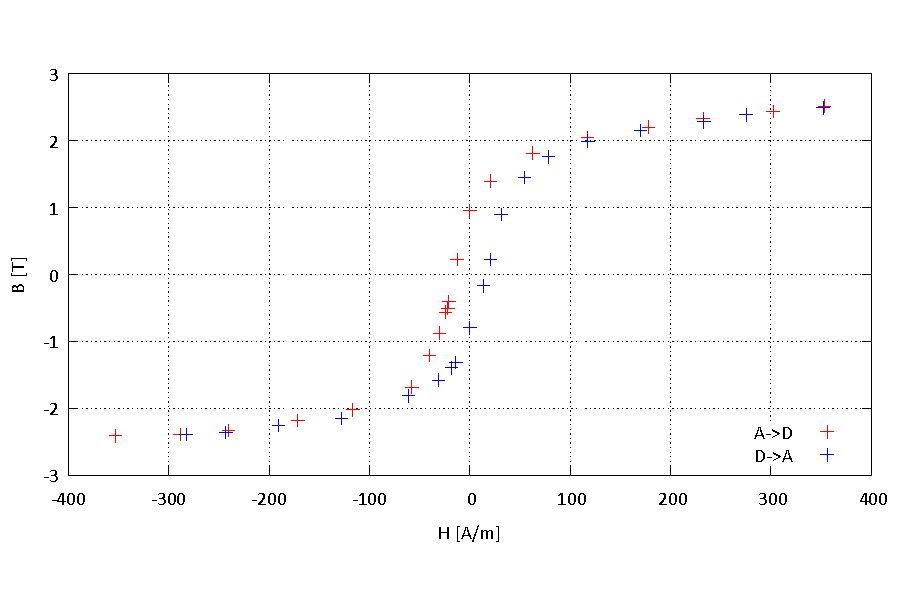
\includegraphics[width=\linewidth]{../gnuplot/hyst.pdf}
	    \vspace*{-2cm}
		\caption{Hysterezní křivka sestavená ze zpracovávaných dat. Posunutí bylo určeno jako aritmetický průměr extrémů obou měření.}
		\label{fig:g_hyst}
	\end{center}
	\end{figure}
%\clearpage
				
%\clearpage
% --- Konec dokumentu --------------------------------------------------


\end{document}

